

\documentclass[]{article}
\usepackage{graphicx}
\usepackage{amsmath}
\usepackage{amssymb}
\usepackage{amsfonts}
\usepackage{fancyhdr}
\usepackage[headheight=65pt,tmargin=150pt,headsep=95pt]{geometry}
\usepackage{ragged2e}
\usepackage{array}
\usepackage{tabularx}
\usepackage{multirow}
\usepackage{booktabs}


%list of images
\graphicspath{{./images/}}

\pagestyle{myheadings}
\markright{Extra Solar Lab Report\hfill 2663452m\hfill 16/1/2023\hfill}

\title{\textbf{Identifying Extra Solar Planets and their Key Features using 
the Doppler Wobble and Planetary Transits Methods}}
\author{2663452m (University of Glasgow)}
\date{16/1/2023}






\begin{document}
\maketitle

\begin{abstract}
In this report, the search for extra-solar planets is discussed,
with emphasis on using the Doppler Wobble and Planetary Transits 
methods to identify extra-solar planets and their key features, 
such as the mass of the planet and the semi-major axis of its orbit.
These methods are effective when observing planets who's orbits 
are close to the plane of the observer's line of sight. For the Doppler 
Wobble method two stars are considered who are known to have
extra-solar planets in orbit around them. The radial velocity of 
the parents stars are measured and thus allowing the mass of the 
planets and the semi-major axis of their orbits to be calculated.
However, for the Planetary transits method, only one star is considered
and to determine the relevant characteristics of the extra-solar planets,
the magnitude of the I-band of the star is measured as a function
of time, and creating a phase-folded light curve.
  



\end{abstract}
\newpage


% All relevant sections for Method 1 (Doppler Wobble)

\twocolumn
\section*{Introduction and Background}
The search for extra-solar planets has been a growing field of Astronomy for the 
past 30 years since the first extra-solar planet was discovered in 1992, this 
detection was made indirectly by observing gaps in a pulsars emission of radio waves.$^1 $
However it wasnt until 1995 that the first direct detection of an extra-solar planet 
via the radial velocity method was made.$^2$ This method is based on measuring the 
wavelength and intensity of light emitted from a star over a period of time, 
from this, a pattern can be seen where, when the star is moving towards the observer
the wavelength of the light emitted is shifted towards the blue end of the 
Electromagnetic spectrum 
(resulting in a lower wavelength) and when the star is moving away from the observer
an increase in wavelength is observed (redshift).$^3$
\par
By measuring the wavelength and intensity and thus the radial velocity of a star as 
a function of time, it is possible to determine characteristics about the Planetary
companions in orbit such as the mass of the planet using Kepler's third law and Newton's
law of Unviersal Gravitation, an equation can derived as seen in equation 1.$^4$
\begin{equation}\label{eq:mass of planet eq}
  v_s = \left(\frac{2\pi G}{T}\right)^{1/3}M_s^{-2/3}m_p
\end{equation}
where $v_s$ is the amplitude of the radial velocity curve (RVC), $G$ is the unviversal
gravitational constant, $T$ is the orbital period of the planet, $M_s$ is the mass of
the star and $m_p$ is the mass of the planet.
\par
From the mass of the planet the semi-major axis of the orbit of the planet can be 
calculated using Kepler's third law as seen in equation 2.$^4$

\begin{equation}\label{eq:semi-major axis eq}
  G(M_s+m_p) = \frac{4\pi^2a^3}{T^2}
\end{equation}
where $a$ is the semi-major axis of the orbit, $G$ is the unviversal gravitational
and the rest of the variables are the same as in equation 1.
\par



\section*{The Doppler Wobble Method of Detecting Extra-solar Planets}
\par
For the analysis on data of two stars and the existence of an extra-solar planets 
around them, the doppler wobble method was used. This method is based on measuring the 
radial velocity of the stars (HD-28185 and HD-73256) as they move towards and away from 
the observer. Thus
producing a doppler shift in the light emitted from the stars, that can be used to 
determine the velocity of the stars in the plane of the observer's line of sight. 
\par
To determine the radial velocity, observations were made of the stars on different
Julian dates, recording the wavelength of light emitted as well as the observed intensity 
of the light. The radial velocity of the stars can then be calculated using the doppler
shifted wavelength and intensity, as provided in the Python Library.$^4$ 
\begin{equation}\label{eq:wavelength doppler}\lambda_{obs} = \lambda_{emit}{(1+v/c)}
\end{equation}

\begin{equation}\label{eq:intensity doppler}I_{obs} = \frac{I_{emit}}{(1+v/c)}
\end{equation}
where $\lambda_{obs}$ is the observed wavelength, $\lambda_{emit}$ is the 
emitted wavelength, $I_{obs}$ is the observed intensity, $I_{emit}$ is the emitted 
intensity, $v$ is the radial velocity of the stars and $c$ is the speed of light.
From this it was possible to calculate the radial velocity of each star on each date.
This was done using the Python SCIPY library.$^5$ An uncertainty in the radial velocity
was assigned to each date of each star of $\pm 15 ms^-1$.$^3$
\par

\begin{figure}[h]
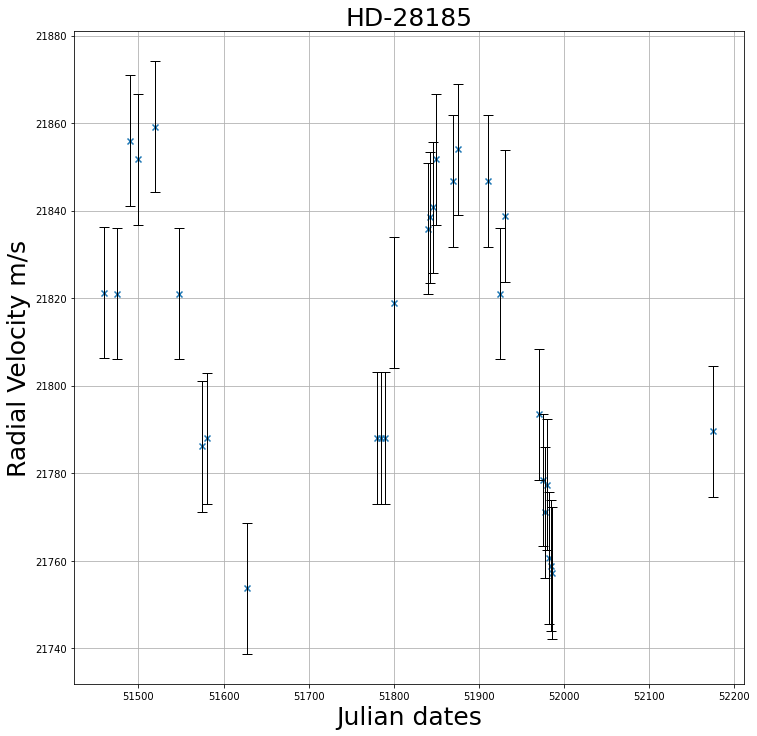
\includegraphics[width=6cm]{images/HD-28185_init.png}
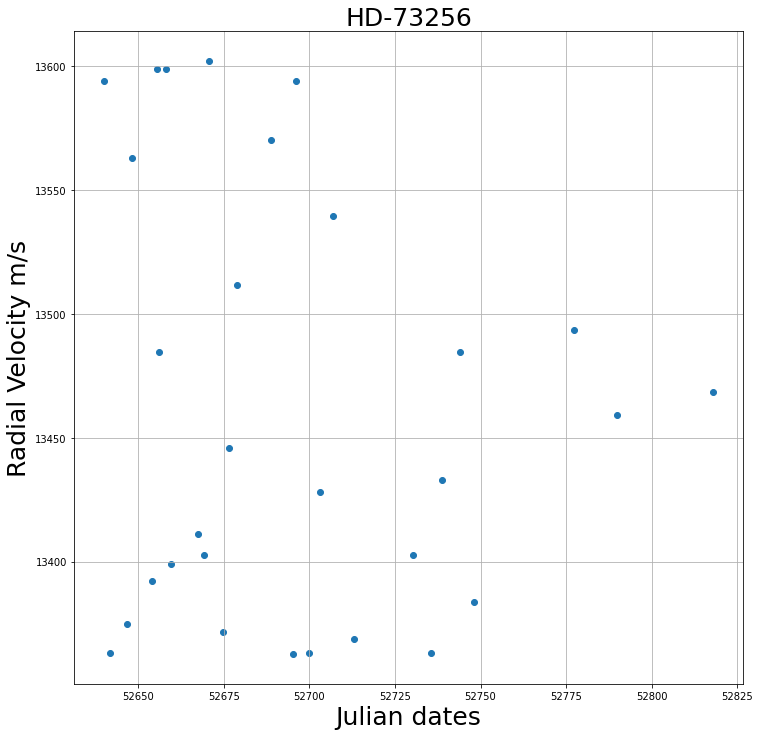
\includegraphics[width=6cm]{images/HD-73256_init.png}
\caption{Radial velocity of HD-28185 and HD-73256 as a function of time (Julian Date)}
\label{fig:HD-_init}
\end{figure}

When plotting the radial velocity as a function of time, as seen in Figure 1, it was
possible to see that there was a periodic sinusoidal pattern in the data, however, 
it was not very accurate as the time between observations varyed.
To correctly plot the radial velocity of the stars over time it was neccessary 
to calculate the phase of each star through the period of the orbit. In this experiment
the phase is defined as the fraction of the orbital period that has elapsed.
The radial velocity of the stars (HD-28185 and HD-73256) as a function of phase 
was then plotted, as seen in Figure 2. This allowed for a more accurate representation
of the radial velocity of the stars as a function of time, as the time between 
observations was more consistent.
\par
\newpage

\begin{figure}[h]
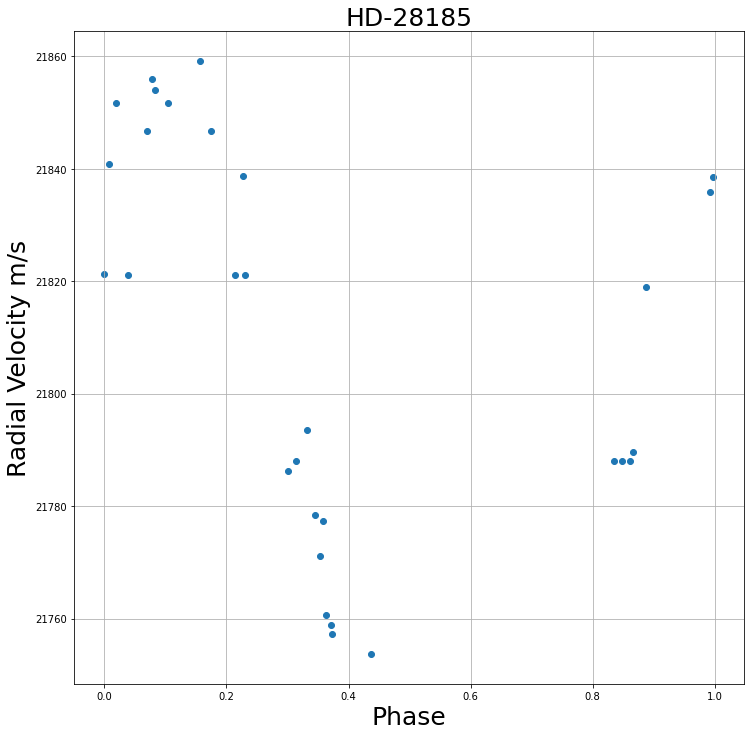
\includegraphics[width=6cm]{images/HD-28185_phase.png}
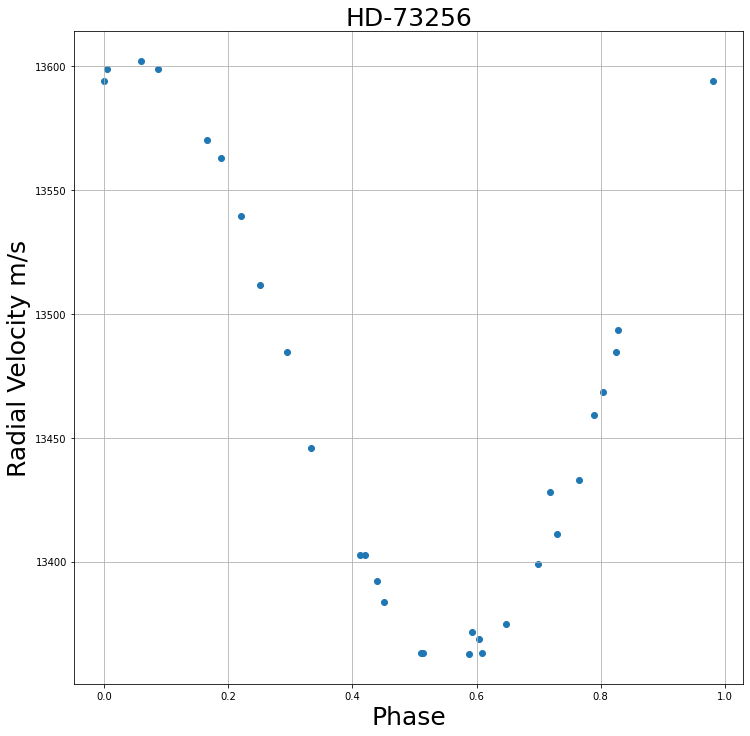
\includegraphics[width=6cm]{images/HD-73256_phase.png}
\caption{Radial velocity of HD-28185 and HD-73256 as a function of phase}
\label{fig:HD-_phase}
\end{figure}

Now that there was a clear correlation between the radial velocity of the stars and
time, it was possible to calculate characteristics about the extra-solar planets in 
orbit around the stars (HD-28185 and HD-73256) using 
\begin{equation}\label{eq:lab book eq2}
  v_{pred} = v_{mean}+v_s\cos[2\pi(\phi_{obs}-\phi_{max})]
\end{equation}


\begin{table*}[t]
  \begin{center}
    \caption{Radial velocities and Phase of stars HD-28185 and HD-73256.}
    \label{tab:table1}
    \begin{tabular}{c|c|c}
       & {HD-28185} & {HD-73256} \\
      \hline
      $v_{mean} $ & $ 2.18\times10^4 \pm4.00ms^{-1}$ & $1.35\times10^4\pm2.80ms^{-1}$ \\
      \hline
      $v_{s}$ & $67.6\pm6.16ms^{-1} $ & $1.20\times10^2\pm3.92ms^{-1}$\\
      \hline
      $\phi_{max}$ & $8.59\times10^{-2} \pm 0.01$ & $5.73\times10^{-2}\pm0.01$  \\
      
    \end{tabular}
  \end{center}
\end{table*}
\begin{table*}[t]
  \begin{center}
    \caption{Mass and semi-major axis of planets in orbit around stars HD-28185 and HD-73256.}
    \label{tab:table2}
    \begin{tabular}{c|c|c}
       & {HD-28185} & {HD-73256} \\
      \hline
      $m_p$ & $1.7654\pm0.1089\times10^{25}kg$ & $1.0517\pm0.0413\times10^{26}kg$ \\
      \hline
      $a$ & $2.2756\pm0.1365\times10^{6}m$ & $2.5446\pm0.1018\times10^{7}m$\\
      
    \end{tabular}
  \end{center}
\end{table*}


By using the data calculated so far in this report it was possible to now calculate 
the mean radial velocity $v_{mean} $, the amplitude of the (RVC)
 $v_{s}$ and the 
phase when the RVC is at a maximum $\phi_{max}$ of the stars.
As well as the associated covariance matrix uncertainties for each of these values.
\par
For the stars (HD-28185 and HD-73256) the values obtained for $v_{mean}$, $v_{s}$ 
and $\phi_{max}$ were.



Values of $\phi_{max}$ are dimensionless in this instance as they are
fractions of the orbital periods.
\par
Now that values for $v_{mean}$, $v_{s}$ and $\phi_{max}$ of both stars have 
been calculated, it was possible to determine the mass and semi-major axis of the
extra-solar planets in orbit around the stars (HD-28185 and HD-73256).
The mass of the planets was calculated using.
\begin{equation}
  v_s = \left(\frac{2\pi G}{T}\right)^{1/3}M_s^{-2/3}m_p \tag{\ref{eq:mass of planet eq}}
\end{equation}
where the mass of the planet $m_p $ is dependent on the amplitude of the RVC $v_{s}$, the mass of the star $M_s$ and the period of the orbit of the planet $T$.
As the mass of the parent star had not been calculated previously it was necessary to
make an educated assumption of what this mass might be. Therefore based on the idea 
that these stars share similar properties to the sun it was assumed that the mass of
the parent stars was $M_s = 1.0M_{\odot}$. Then by rearrangin equation 2 we can 
obtain an equation for a the semi-major axis.
\begin{equation}
  a = \left(\frac{G(M_s+m_p)T^2}{4\pi^2}\right)^{1/3}
  \end{equation}
it was possible to calculate the semi-major axis of the planets in orbit around the
stars (HD-28185 and HD-73256). The values for the mass and semi-major axis of the 
relevant planets around each star are shown in table 2, with the associated 
uncertainties progated from the uncertainties in the values of $v_{mean}$, $v_{s}$
and $T$.


  \par
  
\section*{Conclusion}
From the data collected it is possible to determine that the 
accuracy of the Doppler wobble method is effective at detecting 
extra-solar planets, as, when comparing the two stars (HD-28185 and HD-73256)
with similar masses, their respective planets have 
similar masses and semi-major axis of orbit, giving rise to the 
idea that for a star with a particular mass there is a likely chance
that a planet with a similar mass will be in orbit around it.
\par


% All relevant sections for Planetary transits method

\section*{Introduction and Background}
Searching for Extra-solar planets can be difficult however, 
those orbiting along the plane of the observer can be 
detected using the method of Planetary Transits (PLT).
This method relies on observing the flux from a star and the 
reduction that can be seen when a planet partially blocks some 
area of the star, this reduction in Flux is known as a transit.
However one of the drawbacks of this method is that it relies on 
a telescope with a relatively high angular resolution. 
From this method we can determine the semi-major axis of the planets
orbit and from this the circumference of orbit, the radius of the star
and the radius of the planet.
\par



\section*{The Planetary Transit Method for Detecting Extra-solar Planets}
The Method of Planetary Transits for detecting extra-solar planets
around stars first requires
the magnitude of light from (in this case) the I-band of 
the star to be measured over some period of time.
By plotting the this magnitude of I-band light as a 
function of the phase of the planetary orbit, it is 
possible to observe a significant reduction in the 
magnitude for a short period of time. And thus this can be 
deduced to be the transit of a satellite around the star.
For the star being measured in this report (OGLE-III-TR56)$^4$
the magnitude of light was measured over one orbit of the 
planet (one phase) and the results are shown in Figure 3

\begin{figure}[h]
  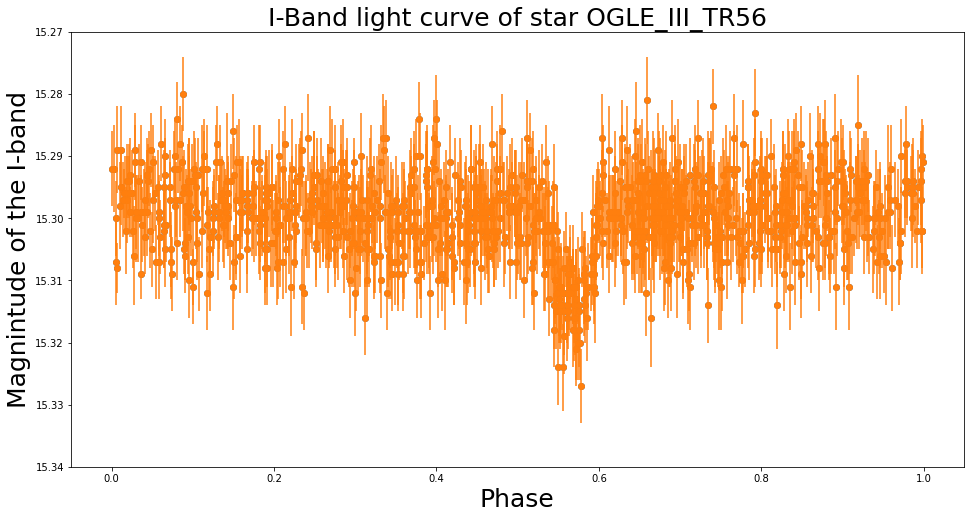
\includegraphics[width=7cm]{images/I-band_curve.png}
  \caption{I-band light as a function of phase for star OGLE-III-TR56}
  \label{fig:HD-_init}
  \end{figure}

To be able to take more accurate data from this graph, it
was necessary to limit the graph to the area of interest 
(the dip in magnitude) as can be seen in Figure 4.

\begin{figure}[h]
  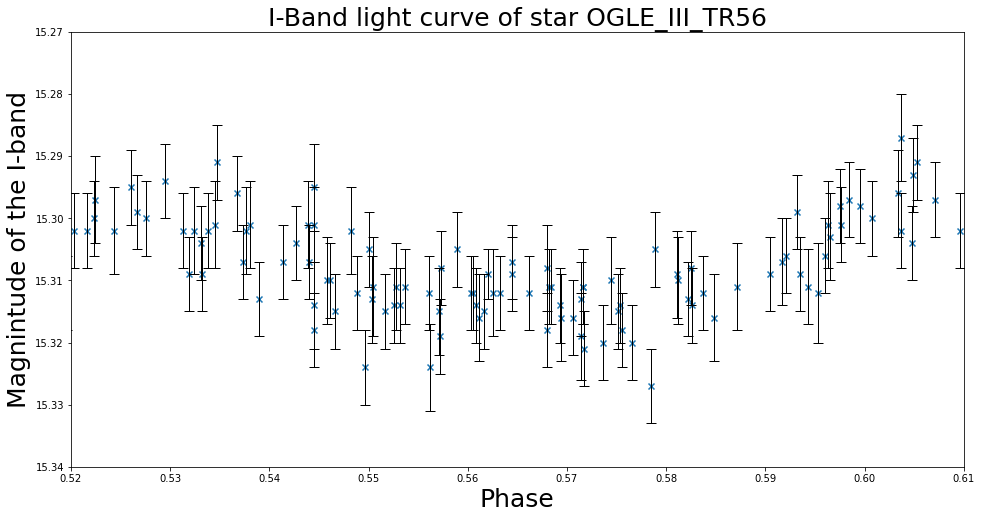
\includegraphics[width=7cm]{images/I-band_limit.png}
  \caption{I-band light as a function of phase for star OGLE-III-TR56
  limited to the dip in magnitude}
  \label{fig:HD-_init}
  \end{figure}

Now that a phase-folded light curve has been obtained,
it is possible to start calculating certain properties
about the Extra-solar Planet that has been detected.
THe first of these properties is the semi-major axis
of the orbit of the planet. This was calculated using the 
Kepler's Third law of Planetary motion as seen below.

\begin{equation}
  G(M_s+m_p) = \frac{4\pi^2a^3}{T^2} \tag{\ref{eq:semi-major axis eq}}
  \end{equation}
As the star that we are observing is roughly equivalent to 1 
solar mass ($1M_\odot $) and other similar characteristics it is reasonable 
to assume that the mass of the planet is equal to 
the mass of the earth and therefore is negligible compared to 
the mass of the star and can be omitted. 
Rearranging equation 2 for $a$ the semi-major axis
gives us:

\begin{equation}
  a = \left(\frac{GM_{\odot}T^2}{4\pi^2}\right)^{1/3}
  \end{equation}
where $G$ is the gravitational constant, $M_\odot$ is the mass of the star,
and $T$ is the period of the orbit of the planet.
From this we can obtain \newline$1.0737\pm0.0179\times10^{8}m $
for the semi-major axis of orbit ($a$).
\par
The next property to calculate was the radius of the planet,
however in order to do this, it was first necessary to calculate 
the circumference of the orbit, which can be done when assuming 
that the orbit is circular and therefore the circumference is 
equal to $2\pi r $, where $r$ is the radius of the orbit.
This gives a value of $6.7460\pm0.1125 \times10^{8}m $
for the circumference of orbit. Now by comparing the fraction 
of the orbital circumference that the planet covers in one orbit, 
the diameter of the star can be calculated by extrapolating 
lines on the graph in Figure 4 like shown in Figure 5.$^4$ 

\begin{figure}[h]
  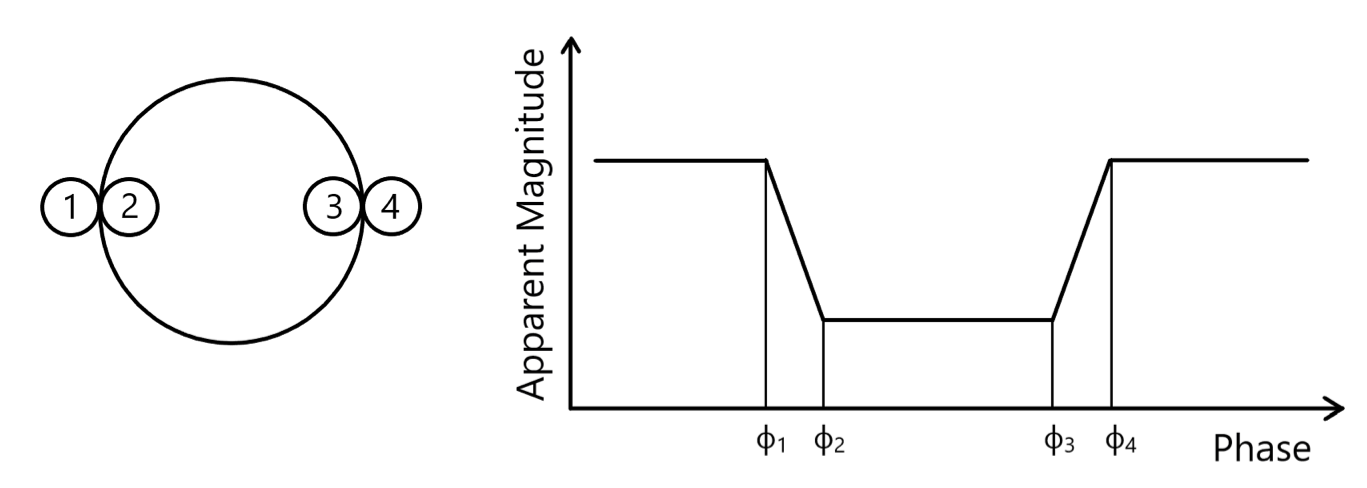
\includegraphics[width=7cm]{images/planet transit of star.png}
  \caption{$\phi_1 $ and $\phi_4$ show where the planet intially covers
   the star as in position 1 and 4 on the left}
  \label{fig:HD-_init}
  \end{figure}

Then by using equation 
\begin{equation}\label{eq: radius of star eq}
  r_s = \frac{0.071C}{2}
  \end{equation}
where $r_s$ is the radius of the star, $C$ is the circumference of the orbit
thus radius of the star is $2.3949\pm0.0399\times10^7m $.
\par
Finally the radius of the planet can be calculated, this is 
simalar to how the radius of the star was calculated but 
by using when the planet starts to eclipses the star as shown by 
position $\phi_1$ and when the planet fully eclipses the star
at $\phi_2$ as shown in Figure 5.
From Figure 4 it was taken that the planet began eclipsing at 0.545 phase
and was fully eclipsing at a phase of 0.553 thus giving a fraction 
of the orbital circumference equal to the diameter of the planet.
using equation \ref{eq: radius of star eq} where the 0.071 is changed 
to 0.08 the diameter of the planet can be found to be $5.3986\pm 0.0900\times10^6m $
\section*{Conclusion}

The Planetary Transits method for detecting extra-solar planets
is an effective method for the initial detection of a planet
assuming that the telescope used has a high enough resolution,  
as the stars intensity as a planet is in transit is reduced by a
significant amount. However, this method appears to be limited due 
to the difficulty of obtaining accurate data from the light curve, 
as from observation it is difficult to determine the exact point 
at which a planet begins to eclipse resulting in a relatively high
uncertainty in the derived values.




\newpage
\onecolumn
\section*{References}

\noindent
[1] {1992 Natur.355..145W,
       author = {{Wolszczan}, A. and {Frail}, D.~A.},
        title = "{A planetary system around the millisecond pulsar PSR1257 + 12}",
      journal = {nat},
     keywords = {Binary Stars, Extrasolar Planets, Orbital Mechanics, Planetary Systems, Pulsars, Accretion Disks, Least Squares Method, Neutron Stars, Radio Astronomy, Supernova Remnants, Astrophysics},
         year = 1992,
        month = jan,
       volume = {355},
       number = {6356},
        pages = {145-147},
          doi = {10.1038/355145a0},
       adsurl = {https://ui.adsabs.harvard.edu/abs/1992Natur.355..145W},
      adsnote = {Provided by the SAO/NASA Astrophysics Data System}

      
}\parskip 0.2cm
\noindent
[2] Mayor, M., Queloz, D. A Jupiter-mass companion to a solar-type star. Nature 378, 355–359 (1995)
. https://doi.org/10.1038/378355a0\parskip 0.2cm



\noindent 
[3] 2022 Extra-solar Planets Lab Record, Lewis McNish\parskip 0.2cm


\noindent
[4] School of Physics and Astrophysics - University of Glasgow, 
Detecting Extrasolar Planets, Astronomy 2 Lab Script, 2022-2023, 9th November 2022\parskip 0.2cm

\noindent
[5] {2020 SciPy-NMeth,
  author  = {Virtanen, Pauli and Gommers, Ralf and Oliphant, Travis E. and
            Haberland, Matt and Reddy, Tyler and Cournapeau, David and
            Burovski, Evgeni and Peterson, Pearu and Weckesser, Warren and
            Bright, Jonathan and {van der Walt}, St{\'e}fan J. and
            Brett, Matthew and Wilson, Joshua and Millman, K. Jarrod and
            Mayorov, Nikolay and Nelson, Andrew R. J. and Jones, Eric and
            Kern, Robert and Larson, Eric and Carey, C J and
            Polat, {\.I}lhan and Feng, Yu and Moore, Eric W. and
            {VanderPlas}, Jake and Laxalde, Denis and Perktold, Josef and
            Cimrman, Robert and Henriksen, Ian and Quintero, E. A. and
            Harris, Charles R. and Archibald, Anne M. and
            Ribeiro, Ant{\^o}nio H. and Pedregosa, Fabian and
            {van Mulbregt}, Paul and {SciPy 1.0 Contributors}},
  title   = {{{SciPy} 1.0: Fundamental Algorithms for Scientific
            Computing in Python}},
  journal = {Nature Methods},
  year    = {2020},
  volume  = {17},
  pages   = {261--272},
  adsurl  = {https://rdcu.be/b08Wh},
  doi     = {10.1038/s41592-019-0686-2},
}
\end{document}